\documentclass{beamer}
\usetheme{metropolis}
\usepackage{booktabs}
\usepackage{tikz}
\usetikzlibrary{arrows.meta, positioning, shapes.geometric, calc}

\title{The Knowledge Lifecycle of Large Language Models}
\subtitle{A Unified Framework for Persistent AI Agents}
\author{Amey Thakur}
\date{Research Presentation, 2026}

\begin{document}

\maketitle

% --- SLIDE 1 ---
\begin{frame}{The Crisis of Fragmentation}
  \begin{itemize}
    \item Current research is siloed into subfields:
    \begin{itemize}
      \item RAG, Knowledge Editing, Continual Learning, Agent Memory.
    \end{itemize}
    \item \textbf{The Problem:} We optimize individual stages but ignore the \textbf{boundaries} between them.
    \item \textbf{Result:} "Boundary Failures" (hallucinations) that no single-stage metric can detect.
  \end{itemize}
\end{frame}

% --- SLIDE 2 ---
\begin{frame}{The Knowledge Lifecycle Framework}
  \centering
  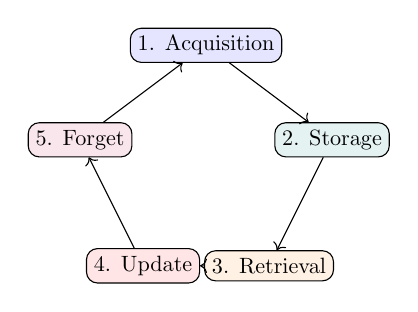
\begin{tikzpicture}[scale=0.8, every node/.style={transform shape}]
    \node[draw, rounded corners, fill=blue!10] (acq) at (0,2) {1. Acquisition};
    \node[draw, rounded corners, fill=teal!10] (sto) at (2,0.5) {2. Storage};
    \node[draw, rounded corners, fill=orange!10] (ret) at (1,-1.5) {3. Retrieval};
    \node[draw, rounded corners, fill=red!10] (upd) at (-1,-1.5) {4. Update};
    \node[draw, rounded corners, fill=purple!10] (fgt) at (-2,0.5) {5. Forget};
    
    \draw[->] (acq) -- (sto);
    \draw[->] (sto) -- (ret);
    \draw[->] (ret) -- (upd);
    \draw[->] (upd) -- (fgt);
    \draw[->] (fgt) -- (acq);
  \end{tikzpicture}
  \vspace{0.3cm}
  \begin{itemize}
    \item A unified view of how knowledge moves through a model.
    \item Focuses on the \textbf{Interactions} between stages.
  \end{itemize}
\end{frame}

% --- SLIDE 3 ---
\begin{frame}{Quantifying the Failure: $\mathcal{D}_{sync}$}
  \begin{itemize}
    \item \textbf{Lifecycle Desynchronisation ($\mathcal{D}_{sync}$):}
    \item Measures information loss when parametric weights ($\theta$) contradict non-parametric context ($\mathcal{M}$).
  \end{itemize}
  \begin{equation*}
    \mathcal{D}_{sync} = D_{KL}(P_{synced} \| P_{stale})
  \end{equation*}
  \begin{itemize}
    \item \textbf{High $\mathcal{D}_{sync} > 1.0$:} Dangerous desynchronisation.
    \item The model "hallucinates" by preferring stale memory over updated context.
  \end{itemize}
\end{frame}

% --- SLIDE 4 ---
\begin{frame}{Solution 1: The Provenance Vector ($p$)}
  \begin{itemize}
    \item \textbf{Proposal:} Append a temporal metadata vector $p_i = [\tau_i; s_i]$ to every FFN value vector.
    \item This makes the model's memory \textbf{Time-Aware}.
  \end{itemize}
  \begin{equation*}
    \text{FFN}(x) = \sum_{i=1}^{d_m} f(x \cdot k_i) [v_i; p_i]
  \end{equation*}
\end{frame}

% --- SLIDE 5 ---
\begin{frame}{Solution 2: Activation Steering}
  \begin{itemize}
    \item During Inference (System 2), the model "mutes" old facts.
  \end{itemize}
  \begin{equation*}
    S(\Delta \tau_i) = \sigma(\beta \cdot \Delta \tau_i - \gamma)
  \end{equation*}
  \begin{itemize}
    \item \textbf{Impact:} The model resolves the conflict dynamically without retraining.
    \item Provenance steering reduces $\mathcal{D}_{sync}$ toward the mathematical lower bound.
  \end{itemize}
\end{frame}

% --- SLIDE 6 ---
\begin{frame}{Case Study: The Vioxx Failure}
  \begin{itemize}
    \item \textbf{Scenario:} Vioxx withdrawn in 2004 due to heart risk.
    \item \textbf{Text-Only Failure:} Model ignores RAG withdrawal notice, predicts "Safe" ($P=42.5\%$).
    \item \textbf{Multimodal Failure:} Model ignores "FDA Withdrawn" visual label due to text-prior override.
    \item \textbf{Result:} High $\mathcal{D}_{sync}$ across modalities.
  \end{itemize}
\end{frame}

% --- SLIDE 7 ---
\begin{frame}{Conclusion: The Future of Agentic AI}
  \begin{itemize}
    \item We cannot rely on static forward-passes for knowledge management.
    \item Epistemic consistency requires a **formal lifecycle**.
    \item \textbf{Roadmap:} Integrate $p$ into pre-training and use $\mathcal{D}_{sync}$ for real-time auditing.
  \end{itemize}
  \vspace{0.5cm}
  \centering \Large \textbf{Questions?}
\end{frame}

\end{document}
